\subsection{Progettazione di dettaglio e codifica}
\textit{\textbf{Periodo}: dal 2021-03-08 al 2021-04-19}

L'inizio di questa fase coincide con la data della Revisione di Progettazione e si conclude con la scadenza della Revisione di Qualifica.

\subsubsection{Obiettivi generali}

\begin{itemize}
\item \textbf{Incremento e verifica documenti}: vengono realizzati gli incrementi necessari ai documenti. I documenti in questione sono:
\begin{itemize}
\item \NdP{};
\item \AdR{};
\item \PdQ{};
\item \PdP{};
\item Glossario.
\end{itemize}
\item \textbf{Product Baseline\ped{G}}: viene realizzata la baseline architetturale del prodotto, in base alla Technology Baseline\ped{G}. Il codice sviluppato precedentemente nel Proof of Concept\ped{G} può essere riutilizzato, se ritenuto corretto per il design architetturale individuato. Viene inoltre redatto l'\textit{Allegato tecnico}\ped{G} per essere inviato e presentato al \CR{} in un colloquio agile.\\
\item \textbf{Manuali}: Durante lo sviluppo della Product Baseline\ped{G} verranno redatti il \MU{} e il \MM. Il primo servirà per fornire istruzioni per l'utilizzo dell'applicazione, il secondo per fornire informazioni necessarie al mantenimento e l'ampliamento del prodotto;
\item \textbf{Consolidamento}: viene realizzata la presentazione da esporre in sede di Revisione di Qualifica e si approfondiscono aspetti lacunari riguardo il progetto.
\end{itemize}

La fase viene suddivisa in sei incrementi, di seguito riportati e spiegati.

\subsubsection{Incremento 5}
\textit{\textbf{Periodo}: dal 2021-03-09 al 2021-03-12}

\myparagraph{Obiettivi}
Gli obiettivi definiti per questo incremento sono i seguenti:
\begin{itemize}
\item incremento della documentazione;
\item preparazione alla progettazione in dettaglio e codifica del prodotto;
\item approfondimento personale per requisiti non sviluppati dal Proof of Concept\ped{G}.
\end{itemize}

\myparagraph{Attività}
Per raggiungere gli obiettivi, vengono svolte le seguenti attività:
\begin{itemize}

\item \textbf{configurazione prodotto}:
\begin{itemize}
\item creazione nuove repository\ped{G} e ambienti di sviluppo;
\item configurazione del prodotto come fatto per Proof of Concept\ped{G}, con opportune correzioni basate sulle segnalazioni del colloquio con proponente e in sede di Technology baseline\ped{G}.
\end{itemize}

\item \textbf{approfondimento tecnologie}:
\begin{itemize}
\item ricerca best practices per le tecnologie da utilizzare;
\item studio di tecnologie mancanti nel Proof of Concept\ped{G}.
\end{itemize}

\item \textbf{ampliamento documentazione e verifiche}:
\begin{itemize}
\item aggiornamento \PdPv{3.0.0} per pianificazione dei successivi incrementi;
\item incremento del \Glossariov{3.0.0};
\item rilevazione e registrazione di metriche, esiti di verifica e obiettivi di qualità;
\item aggiornamento dei rischi rilevati;
\item calcolo e registrazione del consuntivo di periodo.
\end{itemize}

\end{itemize}
\myparagraph{Diagramma di Gantt}

\begin{figure}[H]
\centering

\centerline{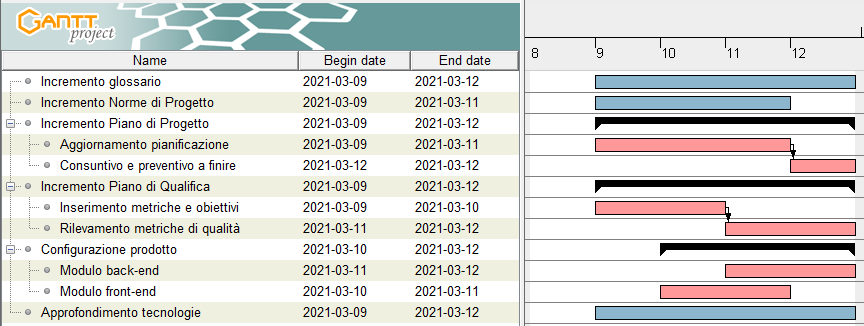
\includegraphics[scale=0.6]{res/Pianificazione/Fasi/CodificaIncrementi/ganttIncremento5}}
\caption{Diagramma di Gantt per l'incremento 5}
\end{figure}


\subsubsection{Incremento 6}
\textit{\textbf{Periodo}: dal 2021-03-13 al 2021-03-17}

\paragraph{Obiettivi}\\
Gli obiettivi definiti per questo incremento sono i seguenti:
\begin{itemize}
\item implementazione autenticazione del sito e visualizzazione pagina del profilo;
\item incremento della documentazione, con correzione in base a segnalazioni dei committenti;
\item inizio stesura di manuali e allegato tecnico.
\end{itemize}

\paragraph{Attività}\\
Per raggiungere gli obiettivi, vengono svolte le seguenti attività:
\begin{itemize}

\item \textbf{codifica}:
\begin{itemize}
\item implementazione UC1 - Registrazione cliente
\item implementazione UC2 - Visualizzazione errori di registrazione
\item implementazione UC3 - Login
\item implementazione UC4 - Visualizzazione errori dati login errati
\item implementazione UC5 - Logout
\item implementazione UC9 - Visualizzazione 
\end{itemize}

\item \textbf{progettazione}:
\begin{itemize}
\item ricerca best practices per le tecnologie da utilizzare;
\item studio di tecnologie mancanti nel Proof of Concept\ped{G}.
\end{itemize}

\item \textbf{ampliamento documentazione}:
\begin{itemize}
\item aggiornamento \PdPv{3.0.0} per pianificazione dei successivi incrementi;
\item incremento del \Glossariov{3.0.0};
\item rilevazione e registrazione degli esiti di verifica e obiettivi di qualità;
\item aggiornamento dei rischi rilevati;
\item calcolo e registrazione del consuntivo di periodo.
\end{itemize}

\end{itemize}
\paragraph{Diagramma di Gantt}\\
\subsubsection{Incremento 7}
\textit{\textbf{Periodo}: dal 2021-03-19 al 2021-03-25}

\myparagraph{Obiettivi}
Gli obiettivi definiti per questo incremento sono i seguenti:
\begin{itemize}
\item implementazione autenticazione della visualizzazione dei prodotti (pagine di listino) e della dashboard venditore;
\item incremento della documentazione;
\end{itemize}

\myparagraph{Attività}
Per raggiungere gli obiettivi, vengono svolte le seguenti attività:
\begin{itemize}

\item \textbf{codifica e pianificazione}:
\begin{itemize}
\item implementazione UC16 - Ricerca nel catalogo digitale;
\item implementazione UC17 - Accesso ad una pagina della categoria;
\item implementazione UC18 - Visualizzazione dei prodotti;
\item implementazione UC19 - Selezione dei prodotti;
\item implementazione UC21 - Filtraggio dei prodotti;
\item implementazione UC23 - Visualizzazione del prodotto;
\item implementazione UC26 - Accesso alla merchant dashboard;
\item implementazione UC27 - Inserimento prodotto;
\item implementazione UC28 - Visualizzazione lista prodotti;
\item implementazione UC29 - Modifica prodotto;
\item implementazione UC30 - Rimozione prodotto;
\item implementazione UC31 - Visualizzazione lista categorie;
\item implementazione UC31 - Inserimento categoria;
\item implementazione UC32 - Rimozione categoria;
\item implementazione UC35 - Visualizzazione collegamenti a sistemi di gestione.
\item creazione diagrammi UML inerenti.

\end{itemize}

\item \textbf{ampliamento documentazione e verifiche}:
\begin{itemize}
\item incremento del \MU{} per i casi d'uso implementati;
\item incremento del \MM{} per i casi d'uso implementati;
\item incremento dell'\textit{Allegato tecnico} per i casi d'uso implementati;
\item incremento del \Glossariov{3.0.0};
\item rilevazione e registrazione di metriche, esiti di verifica e obiettivi di qualità;
\item aggiornamento dei rischi rilevati;
\item calcolo e registrazione del consuntivo di periodo.
\end{itemize}

\end{itemize}
\myparagraph{Diagramma di Gantt}
\subsubsection{Incremento 8}
\myparagraph{Consuntivo}

{

\rowcolors{2}{azzurro2}{azzurro3}

\centering
\renewcommand{\arraystretch}{1.8}
\begin{longtable}{C{4cm} C{1.5cm} C{4cm} }

\rowcolor{azzurro1}
\textbf{Ruolo} &
\textbf{Ore}&
\textbf{Costo}\\
\endhead

\textit{Responsabile} & 4 (+0) & 120 (+0\euro{}) \\
\ammProg & 3 (+0) & 60\euro{} (+0\euro{}) \\
\analProg & 0 (+0) & 0\euro{} (+0\euro{}) \\
\progetProg & 13 (+0) & 286\euro{} (+0\euro{}) \\
\programProg & 44 (+0) & 660\euro{} (+0\euro{}) \\
\verifProg & 19 (-1) & 285\euro{} (-15\euro{})\\
\textbf{Totale Preventivo} & \textbf{83} & \textbf{1411\euro{}} \\
\textbf{Totale Consuntivo} & \textbf{82} & \textbf{1396\euro{}} \\
\textbf{Differenza} & \textbf{-1} & \textbf{-15\euro{}} \\


\rowcolor{white}
\caption{Consuntivo di periodo dell'incremento 8}\\

\end{longtable}
}

\myparagraph{Considerazioni}
Il gruppo ha raggiunto gli obiettivi pianificati per questo incremento e l'andamento delle attività non ha subito rallentamenti.\\
Lo sviluppo delle funzionalità, come nell'incremento precedente, non ha trovato ostacoli grossi. Anche la documentazione non ha avuto problemi, permettendo inoltre di utilizzare un'ora in meno per il ruolo di \verifProg{}, data anche l'esperienza accumulata durante il progetto.

\myparagraph{Preventivo a finire}
Il bilancio è positivo rispetto al preventivo dell'incremento, con un risparmio di 15\euro{}, che si va ad aggiungere al bilancio della precedente fase, risultando in un risparmio totale di 21\euro{}.
Gli obiettivi preimpostati sono stati raggiunti a pieno, senza alcun rallentamento rispetto a quanto pianificato.
Alla luce dei costi e degli obiettivi raggiunti, non si ritiene necessaria alcuna ripianificazione degli incrementi o modifica del preventivo.


\subsubsection{Incremento 9}
\textit{\textbf{Periodo}: dal 2021-04-01 al 2021-04-13}

\myparagraph{Obiettivi}
Gli obiettivi definiti per questo incremento sono i seguenti:
\begin{itemize}
\item preparazione alla presentazione della Product baseline\ped{G};
\item incremento della documentazione.
\end{itemize}

\myparagraph{Attività}
Per raggiungere gli obiettivi, vengono svolte le seguenti attività:
\begin{itemize}
\item \textbf{presentazione Product baseline\ped{G}}: creazione e preparazione della presentazione con il \CR{} e con il proponente;
\item \textbf{ampliamento documentazione e verifiche}:
\begin{itemize}
\item incremento del \MU{};
\item incremento del \MM{};
\item completamento dell'\textit{Allegato tecnico} con i diagrammi mancanti;
\item incremento del \Glossariov{3.0.0};
\item rilevazione e registrazione di metriche, esiti di verifica e obiettivi di qualità;
\item aggiornamento dei rischi rilevati;
\item calcolo e registrazione del consuntivo di periodo.
\end{itemize}

\end{itemize}
\myparagraph{Diagramma di Gantt}
\begin{figure}[H]
\centering

\centerline{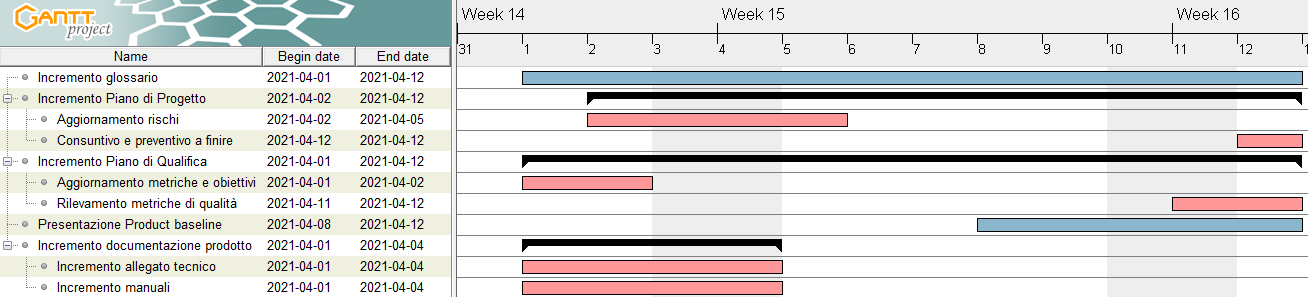
\includegraphics[scale=0.5]{res/Pianificazione/Fasi/CodificaIncrementi/ganttIncremento9}}
\caption{Diagramma di Gantt per l'incremento 9}
\end{figure}
\subsubsection{Incremento 10}
\myparagraph{Consuntivo}

{

\rowcolors{2}{azzurro2}{azzurro3}

\centering
\renewcommand{\arraystretch}{1.8}
\begin{longtable}{C{4cm} C{1.5cm} C{4cm} }

\rowcolor{azzurro1}
\textbf{Ruolo} &
\textbf{Ore}&
\textbf{Costo}\\
\endhead

\textit{Responsabile} & 3 (+0) & 90 (+0\euro{}) \\
\ammProg & 3 (+0) & 60\euro{} (+0\euro{}) \\
\analProg & 0 (+0) & 0\euro{} (+0\euro{}) \\
\progetProg & 4 (+0) & 88\euro{} (+0\euro{}) \\
\programProg & 10 (+0) & 150\euro{} (+0\euro{}) \\
\verifProg & 13 (+0) & 195\euro{} (+0\euro{})\\
\textbf{Totale Preventivo} & \textbf{33} & \textbf{583\euro{}} \\
\textbf{Totale Consuntivo} & \textbf{33} & \textbf{583\euro{}} \\
\textbf{Differenza} & \textbf{+0} & \textbf{+0\euro{}} \\


\rowcolor{white}
\caption{Consuntivo di periodo dell'incremento 10}\\

\end{longtable}
}

\myparagraph{Considerazioni}


\myparagraph{Preventivo a finire rispetto alla fase}

\myparagraph{Preventivo a finire complessivo}





\subsubsection{Diagramma di Gantt}

\begin{figure}[H]
\centering

\centerline{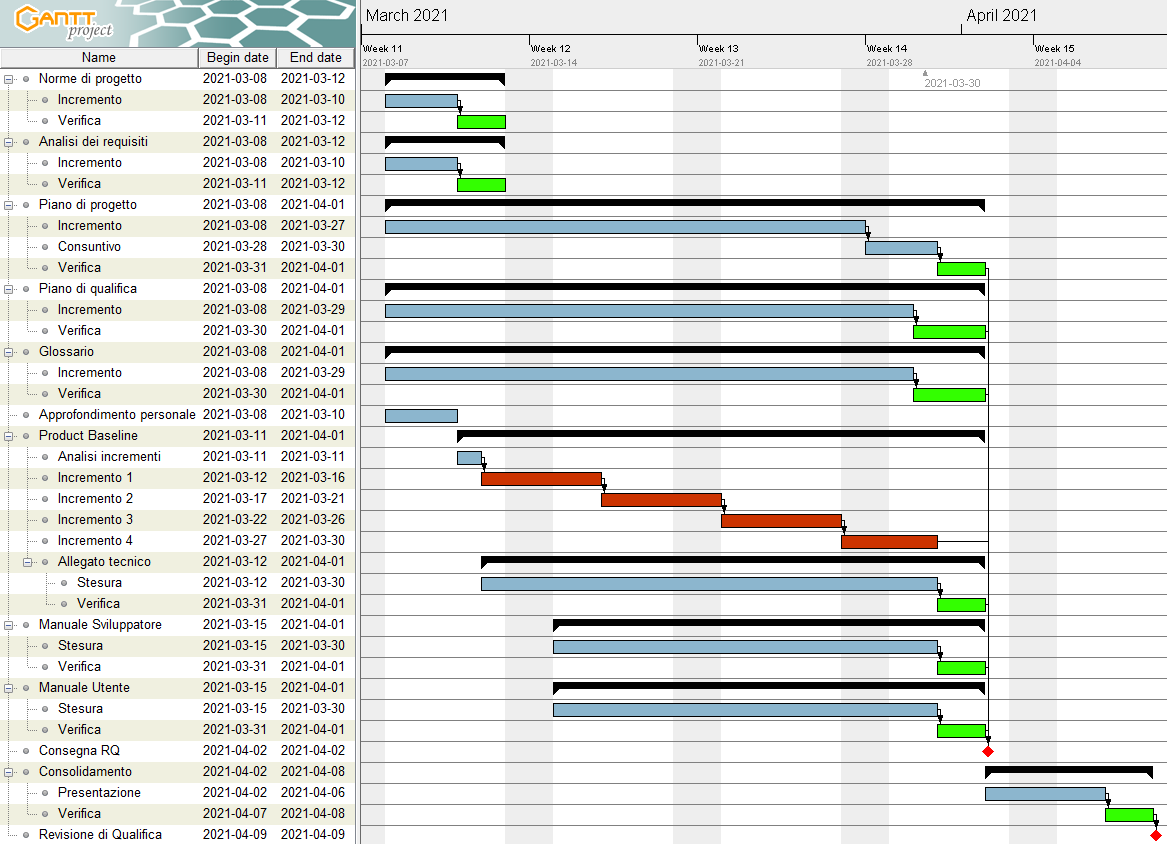
\includegraphics[scale=0.6]{res/Pianificazione/Gantt/codifica}}
\caption{Diagramma di Gantt per il periodo di progettazione di dettaglio e codifica}
\end{figure}
